\documentclass[12pt,paperletter, reqno]{amsart}

%%%%%%%%%%%%%%%%%%%%%%%%%%%%%%%%%%%%%%%%%%%%%%%%%%%%%%%%%%
%%
%% MARK: Packages and Macros
%%
%%%%%%%%%%%%%%%%%%%%%%%%%%%%%%%%%%%%%%%%%%%%%%%%%%%%%%%%%%

\usepackage[utf8]{inputenc}
\usepackage[T1]{fontenc}
\usepackage[french]{babel}
\usepackage{amssymb,amsmath}
\usepackage{graphicx}
\usepackage{url}

% Macros for vectors and fields
\newcommand{\rr}{\mathbf{r}}
\newcommand{\vv}{\mathbf{v}}
\newcommand{\LL}{\mathbf{L}}
\newcommand{\EE}{\mathbf{E}}
\newcommand{\RR}{\mathbf{R}}
\newcommand{\CC}{\mathbf{C}}
\newcommand{\ZZ}{\mathbf{Z}}

% Text shortcuts
\newcommand{\cad}{c'est-\`a-dire}
\newcommand{\ie}{\textit{i.e.}}

% Theorem environments
\theoremstyle{plain}
\newtheorem{theoreme}{Théorème}

\theoremstyle{remark}
\newtheorem*{remarque*}{Remarque}
\newtheorem*{note}{Note}

\parindent 0mm
\parskip .5ex plus 2pt

\usepackage{microtype}
\usepackage[cal=scr,frenchmath,uppercase = upright,greeklowercase = upright,greekfamily = didot, utopia]{mathdesign}

\linespread{1.1}


%%%%%%%%%%%%%%%%%%%%%%%%%%%%%%%%%%%%%%%%%%%%%%%%%%%%%%%%%%
%%
%% MARK: Header
%%
%%%%%%%%%%%%%%%%%%%%%%%%%%%%%%%%%%%%%%%%%%%%%%%%%%%%%%%%%%

\title[Les origines du calcul symplectique]{Les origines du calcul symplectique \\ chez Lagrange}

\author{Patrick Iglesias-Zemmour}
\address{Originated in CMI \\ 39 rue F. Joliot-Curie \\ 13453 Marseille Cedex 13}
\address{Current address: Einstein Institute of Mathematics,
The Hebrew University of Jerusalem,
Campus Givat Ram,
9190401 Israel.}
\email{piz@math.huji.ac.il}
\urladdr{http://math.huji.ac.il/~piz}

\date{\today}

\begin{document}
  
  \maketitle
  
  %%%%%%%%%%%%%%%%%%%%%%%%%%%%%%%%%%%%%%%%%%%%%%%%%%%%%%%%%%
  %%
  %% MARK: Introduction
  %%
  %%%%%%%%%%%%%%%%%%%%%%%%%%%%%%%%%%%%%%%%%%%%%%%%%%%%%%%%%%
  
  \section*{Introduction}
  
  Entre 1808 et 1811,
  Lagrange développe une \emph{théorie de la variations des constantes} appliquée aux problèmes de la mécanique.
  C'est l'acte de naissance du calcul \emph{symplectique},
  terme qui ne sera inventé qu'en 1946 par Hermann Weyl\footnote{Voir la note historique 2 à la fin de cette introduction.}.
  Le but qu'il poursuit à l'époque est la généralisation d'un théorème de Laplace,
  sur la stabilité séculaire du grand axe de l'orbite elliptique d'une planète,
  perturbée par l'attraction d'autres corps célestes.
  
  Depuis Kepler on sait \emph{résoudre} explicitement le problème des éphémérides des planètes.
  C'est-à-dire,
  calculer avec une précision aussi grande que l'on veut la position de la terre (ou de toute autre planète) connaissant sa position et sa vitesse à un instant donné,
  à condition toutefois de considérer seulement l'attraction du soleil et de négliger complètement l'influence des autres planètes.
  Mais bien que ce savoir soit important,
  il est largement insuffisant pour ce qui est du mouvement réel des planètes.
  L'influence des autres planètes sur la terre est-elle vraiment négligeable,
  ne va-t-elle pas à terme déstabiliser notre trajectoire et nous expulser aux confins de l'espace ?
  
  Il faut donc traiter le problème dans sa globalité :
  calculer la position d'une planète quelconque,
  connaissant les positions et vitesses de toutes les planètes,
  et ne négligeant l'influence d'aucune d'entre elles.
  La difficulté de cette question donne le vertige,
  et on ne sait y répondre,
  encore actuellement,
  ni analytiquement ni même numériquement.
  
  On pourrait croire,
  en effet,
  qu'avec l'avènement de l'ordinateur cette question soit devenue académique :
  pourquoi ne pas intégrer naïvement les équations du mouvement par une méthode numérique quelconque.
  Malheureusement,
  si les erreurs d'approximations,
  inévitables dans ce genre de calcul,
  sont négligeables sur un bref intervalle de temps,
  elles deviennent catastrophiques à long terme.
  Cette incertitude sur la position de la planète n'a rien à voir avec une éventuelle situation chaotique du système (le système à deux corps est d'ailleurs parfaitement \emph{intégrable} dans tous les sens raisonnables que l'on veut bien donner à ce mot),
  elle est simplement la conséquence de l'accumulation des erreurs commises par l'ordinateur lors de l'intégration numérique des équations du mouvement.
  L'existence d'une méthode analytique d'intégration du mouvement est donc capitale pour résoudre convenablement cette question.
  Si cette remarque est vraie pour le problème à deux corps,
  elle l'est \emph{a fortiori} pour le problème à $n$ corps (\ie\ un nombre quelconque de planètes en interactions).
  Or,
  comme nous l'avons déjà dit,
  nous ne connaissons toujours aucune méthode analytique satisfaisante susceptible de résoudre cette question.
  Lagrange a contourné cette difficulté en appliquant de façon astucieuse sa méthode de \emph{la variation des constantes} aux problèmes de la mécanique analytique.
  Décrivons rapidement ce dont il s'agit.
  
  Considérons d'abord un corps matériel (une planète) attiré par un centre fixe (le soleil) selon la loi de la gravitation universelle.
  Les équations différentielles qui décrivent son mouvement sont de degré deux dans l'espace à trois dimensions,
  il faudra donc six \emph{constantes d'intégration}\footnote{A cette époque on disait \emph{constantes d'intégration} quand nous parlons aujourd'hui d'\emph{espace de solutions}. Par exemple, l'équation différentielle ordinaire réelle $dx/dt=x$ a toutes ses solutions de la forme $x(t)=c\exp(t)$, où $c$ est une constante arbitraire --- la fameuse constante d'intégration. Or $c$ caractérise justement cette solution.} pour le décrire.
  D'après Newton,
  nous savons que la trajectoire de ce corps est une ellipse\footnote{Si Kepler a découvert le mouvement elliptique des planètes, c'est Newton qui l'a \og déduit\fg{} de la loi de la gravitation universelle qui porte son nom. Pour une discussion plus approfondie sur ce sujet voir la thèse de F. de Gandt \cite{deGandt1}.},
  de foyer le centre d'attraction\footnote{Les caractéristiques géométriques de cette ellipse étant, par ailleurs, liées aux position et vitesse initiales du corps.}.
  Pour décrire complètement cette ellipse il nous faut d'abord connaître le plan dans lequel elle s'inscrit (le plan de l'orbite),
  on peut le repérer par le vecteur unitaire qui lui est orthogonal,
  ce qui fait deux paramètres.
  Pour définir l'ellipse dans son plan on peut choisir la position du deuxième foyer,
  ce qui donne deux nouveaux paramètres,
  et la longueur de l'ellipse\footnote{Il est possible maintenant de tracer l'ellipse par la méthode du jardinier.},
  soit au total :
  cinq paramètres pour situer et décrire la trajectoire du corps dans l'espace.
  
  Mais si ces cinq paramètres suffisent à définir complètement la trajectoire du corps céleste,
  ils ne suffisent pas à déterminer son \emph{mouvement}.
  En effet,
  comment déterminer la position de la planète à chaque instant sur sa trajectoire si nous ne connaissons pas sa position à une origine des temps arbitraire ?
  Ou encore la date de son passage à l'aphélie ?
  Voilà comment s'introduit ce sixième paramètre que les astronomes appellent l'\emph{époque}.
  
  Nous aurions pu tout aussi bien choisir six autres paramètres :
  par exemple les position et vitesse initiales de la planète à l'origine des temps.
  Ils définissent aussi,
  de façon unique,
  le mouvement de la planète.
  Seul le caractère pratique de tel ou tel ensemble de paramètres peut déterminer notre choix.
  Les astronomes appellent \emph{éléments képleriens} de la planète un tel ensemble de six paramètres servant à caractériser son mouvement,
  cinq pour la figure de l'ellipse et l'époque.
  
  L'ensemble des mouvements de la planète considérés indépendamment du choix des paramètres qui nous servent à les décrire\footnote{On dit que c'est une variété.} sera appelé \emph{espace des mouvements képleriens}.
  
  Supposons maintenant que la planète,
  qui suit un mouvement képlerien $m$,
  subisse un choc instantané dû à l'impact d'un astéroïde.
  Après le choc elle suivra encore un mouvement képlerien $m'$ différent du précédent.
  Le mouvement (perturbé) de cette planète sera donc décrit par son mouvement $m$ avant le choc,
  son mouvement $m'$ après le choc et l'instant du choc $t$.
  Supposons ensuite que la planète subisse une série de chocs de ce type.
  Le mouvement réel de la planète sera décrit par une courbe dans l'espace des mouvements képleriens,
  discontinue et constante par morceaux,
  chaque morceau de courbe décrivant le mouvement képlerien de la planète entre deux chocs successifs.
  En étendant ce raisonnement,
  Lagrange assimilera l'interaction des autres planètes du système à une série infinie de chocs \og infiniments petits et continuels\fg{}.
  Il décrira ainsi le mouvement réel de la planète perturbée par une courbe,
  cette fois différentiable,
  tracée dans son espace des mouvements képleriens.
  C'est en précisant l'équation différentielle de cette courbe\footnote{Aujourd'hui cette équation porte le nom d'\emph{équation de Hamilton}, mais pour la petite histoire sachez que Sir W.R. Hamilton avait juste six ans lorsque Lagrange la publia pour la première fois.} qu'il fera apparaître la structure symplectique de l'\emph{espace des mouvements}.
  Il donnera l'expression des composantes de la forme symplectique de l'espace des mouvements képleriens dans le système de coordonnées que sont les \emph{éléments de la planète}.
  Il en déduira entre autre la stabilité séculaire du grand axe des planètes.
  
  J'ai essayé,
  dans cet article,
  d'être le plus fidèle possible aux textes de Lagrange.
  Désirant par là mettre en évidence le processus qui lui a permis,
  en voulant résoudre le problème du système des planètes,
  d'élaborer les premiers éléments de calcul symplectique.
  
  \begin{note}
    C'est le 22 août 1808 que Lagrange présente à l'Institut de France son \emph{Mémoire sur la théorie des variations des éléments des planètes} \cite{Lagrange2} où sont définis pour la première fois les \emph{crochets} et \emph{parenthèses} qui portent son nom et qui sont,
    en termes modernes,
    les composantes de la \emph{forme symplectique} de l'espace des mouvements d'une planète.
    
    Ce mémoire sera suivi de celui \emph{Sur la théorie générale de la variation des constantes arbitraires} \cite{Lagrange3} présenté le 13 mars 1809,
    où il généralise sa méthode à tous les problèmes de mécanique.
    Il en donnera une version notablement simplifiée,
    et définitive,
    le 19 février 1810 \cite{Lagrange4}.
    C'est à partir de cette version qu'il écrira les chapitres relatifs à ces questions dans la deuxième édition de son \emph{Traité de Mécanique Analytique} \cite{Lagrange1} (seconde partie, de la cinquième à la septième section).
    Ce volume ne sera publié qu'après sa mort.
  \end{note}
  
  \begin{note}
    Dans son ouvrage sur \emph{Les Groupes classiques} \cite{Weyl1},
    Hermann Weyl baptise ainsi :
    \emph{groupe symplectique},
    le groupe des transformations linéaires de $\RR^{2n}$ qui préservent la forme bilinéaire antisymétrique $\omega = \sum_{i=1}^n dp_i\wedge dq_i$.
    Les relations étroites entre la structure définie par $\omega$ et la structure complexe ($\RR^{2n}\sim \CC^n$) lui fait choisir le mot \emph{symplectique} [gr. sum-plektikos],
    transposition de \emph{complexe} [lat. com-plexus] pour désigner ce groupe ;
    le mot \emph{complexe} étant par ailleurs réservé.
    Le suffixe \emph{plekticos} $\sim$ \emph{plexus} signifiant \emph{tenir},
    \emph{entrelacer}\ldots
    L'idée de \emph{complexe},
    comme \emph{symplectique} sous-entend l'existence de plusieurs types d'objets (ici deux) maintenus ensemble dans une même structure.
    De façon rapide et en anticipant sur la suite,
    on peut dire que dans le premier cas la \emph{complexité} représente la dualité \emph{réel--imaginaire},
    et dans le second la \emph{symplecticité} représente la dualité \emph{position--vitesse}.
    Voilà ce qu'en dit lui même Weyl \cite[p. 165]{Weyl1} :
    
    \begin{quote}
      The name ``complex group'' formerly advocated by me in allusion to line complexes, as these are defined by the vanishing of antisymetric bilinear forms, has become more and more embarrassing through collission with the word ``complex'' in the connotation of complex number. I therefore propose to replace it by the corresponding Greek adjective ``symplectic''. Dickson calls the group the ``Abelian linear group'' in homage to Abel who first studied it.
    \end{quote}
    
    En ce qui concerne la notion actuelle de \emph{géométrie symplectique},
    au sens de l'étude des variétés différentielles munies d'un forme symplectique,
    il semble que ce soit J.-M. Souriau qui l'ait introduite en 1953 dans son article \emph{Géométrie symplectique différentielle. Applications.} \cite{Souriau20}.
    Dans un article plus récent du même auteur :
    \emph{La structure symplectique de la mécanique décrite par Lagrange en 1811} \cite{Souriau9} on peut lire un autre aspect des relations entre la géométrie symplectique et la mécanique de Lagrange.
  \end{note}
  
  %%%%%%%%%%%%%%%%%%%%%%%%%%%%%%%%%%%%%%%%%%%%%%%%%%%%%%%%%%
  %%
  %% MARK: Géométrie des mouvements
  %%
  %%%%%%%%%%%%%%%%%%%%%%%%%%%%%%%%%%%%%%%%%%%%%%%%%%%%%%%%%%
  
  \section{Géométrie des mouvements d'une planète autour d'un centre fixe}
  
  Pour comprendre et apprécier la méthode de la variation des constantes développée par Lagrange,
  il est nécessaire de bien connaître la résolution du problème à deux corps.
  Nous allons en donner un bref résumé dans ce qui suit.
  
  %%###########
  %\begin{figure}[ht]
  %\centerline{\includegraphics{Figures/Newton.pdf}}
  %\caption{Isaac Newton}\label{Newton}
  %\end{figure}
  %%###########
  
  Depuis Newton on sait que les mouvements d'un point matériel (une planète) autour d'un centre fixe (le soleil) est décrit par l'équation différentielle\footnote{Il faudrait en toute rigueur multiplier $\rr$ par la constante d'attraction solaire, mais nous choisirons les unités de telle sorte qu'elle soit égale à 1.} suivante :
  %
  \begin{equation}
    \frac{d^2\rr}{dt^2} = - \frac{\rr}{r^3},
  \end{equation}
  %
  où $\rr$ désigne un vecteur non nul de l'espace $\RR^3$ et $r$ son module.
  Transformons cette équation différentielle en un système du premier ordre dans $[\RR^3-\{0\}]\times \RR^3$,
  les \emph{mouvements} de la planète deviennent les solutions de :
  %
  \begin{equation}
    \frac{d\rr}{dt}= \vv \qquad \frac{d\vv}{dt}= - \frac{\rr}{r^3}.
  \end{equation}
  %
  Comme on le sait\footnote{depuis Huygens, dans son \emph{Horlogium oscillatorium} de 1673.},
  l'énergie totale du système est conservée le long du mouvement.
  Les astronomes appellent \emph{constante des forces vives} le double de l'énergie,
  on la notera $f$ :
  %
  \begin{equation}
    f = {v^2} - \frac{2}{r}.
  \end{equation}
  %
  D'autre part,
  comme la force d'attraction gravitationnelle est centrale,
  le moment cinétique $\LL$ est lui aussi conservé :
  %
  \begin{equation}
    \LL=\rr\wedge \vv.
  \end{equation}
  %
  De cette invariance on déduit que le mouvement de la planète s'effectue dans le plan orthogonal à $\LL$.
  
  %###########
  \begin{figure}[t]
    \centerline{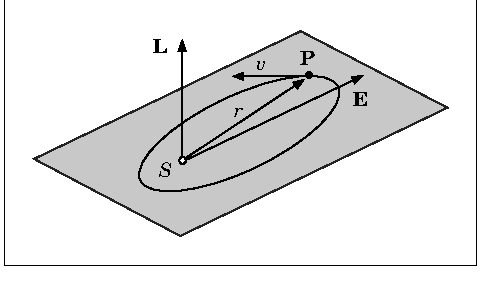
\includegraphics{Figures/IglesiasFig1.pdf}}
    \caption{L'orbite de la planète P}\label{FigOrbite}
  \end{figure}
  %###########
  
  On peut vérifier qu'un autre vecteur,
  indépendant de $\LL$,
  est miraculeusement conservé le long du mouvement,
  c'est \emph{le vecteur de Laplace} :
  %
  \begin{equation}
    \EE=\LL\wedge \vv +\frac{\rr}{r}.
  \end{equation}
  %
  On déduit,
  de cet invariant supplémentaire,
  les trajectoires des planètes.
  En effet,
  on a immédiatement :
  %
  \begin{equation}\label{EqEL}
    E^2=1+fL^2 \quad \mbox{et} \quad \EE.\LL=0.
  \end{equation}
  %
  Le vecteur $\EE$ est donc dans le plan du mouvement.
  On a de plus,
  le long du mouvement :
  %
  \begin{equation}
    \EE.\rr+L^2=r.
  \end{equation}
  %
  Soit $\phi$ l'angle entre $\EE$ et $\rr$,
  alors :
  %
  \begin{equation}
    E r\cos\phi+L^2=r \quad \mbox{ou encore} \quad r=\frac{L^2}{1-E\cos\phi},
  \end{equation}
  %
  On reconnait ainsi l'équation d'une conique de paramètre $L^2$,
  d'excentricité $E$ et d'axe la direction du vecteur $\EE$.
  Les astronomes appellent l'angle $\phi$ l'\emph{anomalie vraie}\footnote{Dans ce contexte, le terme \emph{anomalie} signifie simplement \emph{paramètre}}.
  Le vecteur $\EE$ pourrait s'appeler le \emph{vecteur d'excentricité}.
  
  Les trajectoires de la planète sont donc des sections coniques,
  avec le soleil pour foyer.
  Leur nature dépend essentiellement du signe de l'énergie totale,
  comme le montre la formule (\ref{EqEL}).
  
  \begin{itemize}
    \item Si $f<0$ alors $E<1$, l'orbite est elliptique.
    \item Si $f=0$ alors $E=1$, l'orbite est parabolique.
    \item Si $f>0$ alors $E>1$, l'orbite est hyperbolique.
  \end{itemize}
  
  Dans le cas des orbites elliptiques,
  on trouve tout de suite la valeur du demi-grand axe,
  noté $a$ :
  %
  \begin{equation}
    a = -\frac{1}{f}.
  \end{equation}
  %
  Nous pouvons décrire complètement la variété des mouvements képleriens elliptiques ($f<0$) si l'on exclut les chutes sur le centre,
  \cad\ si on se restreint à $\LL\neq 0$.
  Une trajectoire elliptique est bien définie par les deux vecteurs $\LL$ et $\EE$ ;
  le vecteur $\EE$ donnant à la fois l'excentricité et l'axe de la conique,
  le plan étant défini comme l'orthogonal de $\LL$ et le paramètre de l'ellipse valant $L^2$.
  Autrement dit,
  l'espace des trajectoires képleriennes elliptiques est équivalent à l'ensemble des couples de vecteurs $(\EE,\LL)\in \RR^3\times \RR^3$ tels que :
  %
  \begin{equation}
    E<1, \quad  L\neq 0 \quad \mbox{et} \quad \EE.\LL=0.
  \end{equation}
  %
  C'est une sous-variété,
  de dimension 5,
  de $\RR^3\times \RR^3$.
  Ce n'est pas encore l'espace des mouvements képleriens :
  il nous faut pouvoir calculer la position de la planète à chaque instant.
  On pourrait,
  pour cela,
  choisir la position de la planète sur son orbite (\cad\ l'anomalie vraie) à l'\emph{instant zéro}.
  Mais ce choix donne lieu à des calculs pénibles.
  On considère plutôt le vecteur qui joint l'origine du cercle circonscrit à l'ellipse,
  au point $\mathbf{A}$ de ce cercle qui a la même projection orthogonale,
  sur l'axe dirigé par $\EE$,
  que la planète $P$ (voir figure \ref{FigAExc}).
  
  %###########
  \begin{figure}[ht]
    \centerline{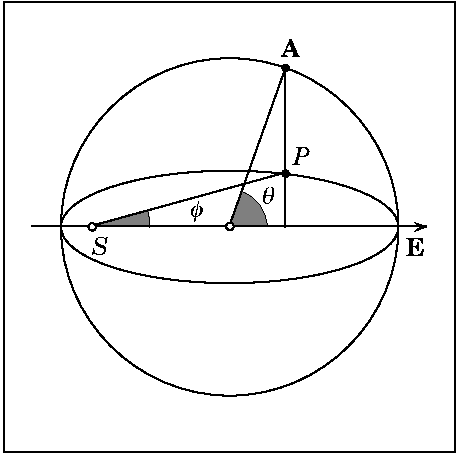
\includegraphics{Figures/IglesiasFig2.pdf}}
    \caption{L'anomalie excentrique}\label{FigAExc}
  \end{figure}
  %###########
  
  Ce vecteur,
  ou plus précisément l'angle $\theta$ qu'il fait avec l'axe de l'ellipse,
  est appelé \emph{anomalie excentrique}\footnote{Comme le montre la figure l'\emph{anomalie excentrique} doit son nom à ce qu'il est le paramètre excentré de l'ellipse, le vrai centre étant bien entendu le foyer : centre d'attraction.},
  il a été introduit par Kepler.
  En utilisant la définition de la constante $f$ et après quelques manipulations algébriques,
  on peut constater que,
  le long du mouvement :
  %
  \begin{equation}
    dt = \sqrt{a^3}\left[\vphantom{\sqrt{a^3}}1-E \cos(\theta)\right] d\theta.
  \end{equation}
  %
  Ce qui nous donne par intégration une nouvelle constante du mouvement :
  %
  \begin{equation}\label{eqKepler}
    c = t - \sqrt{a^3}\left[\vphantom{\sqrt{a^3}}\theta -E \sin(\theta)\right].
  \end{equation}
  %
  C'est la valeur de $t$ pour $\theta =0$,
  \cad\ la date du passage de la planète à l'aphélie.
  C'est ce paramètre que les astronomes appellent l'\emph{époque} de la planète,
  et qu'ils choisissent à la place de l'anomalie excentrique à l'instant zéro\footnote{En réalité ce paramètre est mal défini puisque le mouvement de la planète est périodique. Il n'est vraiment défini que modulo $\sqrt{a^3}$ (la période du mouvement). Il faudrait plutôt choisir $C=\exp(2i\pi c/\sqrt{a^3})$. Ce qui est équivalent au choix de $\mathbf{A}$ à l'instant zéro.}.
  
  \begin{remarque*}
    Les mouvements képleriens sont donc définis par les valeurs de l'époque,
    du moment cinétique et du vecteur de Laplace.
    Mais il est évident,
    puisque tous les mouvements elliptiques sont périodiques,
    que cet espace des mouvements képleriens est aussi l'ensemble des conditions initiales à l'instant $t=0$,
    \cad\ l'ouvert de $\RR^3\times \RR^3$ des couples $(\rr,\vv)$ vérifiant :
    %
    \begin{equation}
      \rr\wedge \vv\neq 0 \quad \mbox{et} \quad v^2 - \frac{2}{r}  <0.
    \end{equation}
    %
    La représentation d'un mouvement képlerien par ses conditions initiales ou par ses caractéristiques géométriques est \emph{a priori} purement affaire de goût.
    Nous verrons quand même que certaines représentations sont plus pratiques que d'autres.
    Lagrange choisira les six \emph{éléments képleriens} $(a,b,c,h,i,k)$,
    où $a$ est la valeur du demi-grand axe (l'inverse de la constante des forces vives au signe près),
    $b$ est le paramètre de l'ellipse (le carré du moment cinétique),
    $c$ est l'époque.
    Les éléments $h$, $i$ et $k$ déterminent le plan de l'orbite et l'axe de l'ellipse dans ce plan :
    $i$ est l'inclinaison du plan de l'orbite par rapport à un plan de référence,
    $h$ est la \emph{longitude des n\oe uds},
    \cad\ l'angle que fait la trace du plan de l'orbite sur le plan de référence (la \emph{ligne des n\oe uds}),
    et $k$ est la \emph{longitude du périhélie},
    \cad\ l'angle que fait l'axe de l'ellipse avec la ligne des n\oe uds.
  \end{remarque*}
  
  
  %%%%%%%%%%%%%%%%%%%%%%%%%%%%%%%%%%%%%%%%%%%%%%%%%%%%%%%%%%
  %%
  %% MARK: La méthode de la variation des constantes
  %%
  %%%%%%%%%%%%%%%%%%%%%%%%%%%%%%%%%%%%%%%%%%%%%%%%%%%%%%%%%%
  
  \section{La méthode de la variation des constantes}
  
  Maintenant que nous avons bien compris et résolu\footnote{En toute rigueur il faudrait encore inverser la fonction $\theta \mapsto t$. Problème connu sous le nom de \emph{Problème de Kepler}. Mais ce n'est pas le but de cet article.} le problème à deux corps (au moins en ce qui concerne les orbites elliptiques),
  il nous reste à traiter le problème à deux corps perturbé,
  et d'introduire ainsi les premiers calculs symplectiques comme l'a fait Lagrange.
  Nous nous bornerons,
  comme lui,
  aux perturbations des orbites elliptiques.
  
  Nous avons déjà expliqué,
  dans l'introduction,
  la méthode de la variation des constantes :
  l'influence de la perturbation à laquelle est soumise une planète attirée par un centre fixe est traduite comme une courbe sur l'espace des éléments de la planète,
  \cad\ l'espace de ses mouvements képleriens.
  C'est cette courbe dont il s'agit de déterminer l'équation,
  et éventuellement d'en extraire quelques renseignements,
  comme par exemple la stabilité du grand axe.
  Ce résultat avait été découvert par Laplace en 1773.
  Nous allons montrer maintenant comment Lagrange l'a inclus dans le cadre général de sa méthode de la variation des constantes.
  
  Supposons donc,
  comme le fait Lagrange,
  que la planète subisse de façon continue une série de chocs infiniment petits.
  Ces chocs se traduisent par une variation instantanée de la vitesse,
  sans conséquence sur sa position.
  Si on désigne par $a$ un élément quelconque de la planète (pas nécessairement le demi grand axe),
  on pourra écrire\footnote{De façon générale, on note $\partial y /\partial x$ l'application linéaire tangente d'une application $x\mapsto y$.} :
  %
  \begin{equation}\label{eq_da}
    \frac{da}{dt} = \frac{\partial a}{\partial \vv}\frac{d\vv}{dt}.
  \end{equation}
  %
  En remarquant que le vecteur $d\vv/dt$ représente exactement la force perturbatrice $X$ exercée sur la planète à l'instant $t$ au point $\rr$,
  la variation infinitésimale de l'élément $a$,
  sous l'effet de la perturbation,
  peut s'écrire à nouveau :
  %
  \begin{equation}\label{eq_B}
    \frac{da}{dt} = \frac{\partial a}{\partial \vv}X.
  \end{equation}
  %
  Le mouvement vrai est ainsi décrit par la courbe intégrale de cette équation,
  tracée dans l'espace des éléments de la planète.
  Cette famille d'ellipses est appelée \emph{famille d'ellipses osculatrices} du mouvement perturbé.
  
  Supposons maintenant que la force perturbatrice $X$ dérive d'un potentiel $\Omega$,
  autrement dit que :
  %
  \begin{equation}
    X = \frac{\partial \Omega}{\partial \rr},
  \end{equation}
  %
  et que ce \emph{potentiel de perturbation} $\Omega$ ne soit fonction que de $\rr$.
  Ce qui,
  dit autrement,
  s'écrit :
  %
  \begin{equation}
    \frac{\partial \Omega}{\partial \vv} =0.
  \end{equation}
  %
  Nous ne changeons donc rien en écrivant :
  %
  \begin{equation}\label{eq_A}
    \frac{da}{dt} = \sum_{i=1}^3\frac{\partial a}{\partial \vv^i}\frac{\partial \Omega}{\partial \rr^i} -  \frac{\partial a}{\partial \rr^i}\frac{\partial \Omega}{\partial \vv^i}.
  \end{equation}
  %
  
  C'est maintenant,
  avec cette transformation astucieuse de Lagrange,
  que la véritable histoire commence,
  d'où sortira la géométrie symplectique.
  Mais allons un peu plus loin :
  puisque l'application $(t,\rr,\vv)\mapsto (t,a,b,c,h,i,k)$ est un difféomorphisme,
  le potentiel de perturbation peut être considéré aussi bien comme une fonction de $\rr$ que comme une fonction du temps $t$ et des éléments $(a,b,c,h,i,k)$ de la planète.
  En remplaçant l'expression de :
  %
  \begin{equation}
    \frac{\partial \Omega}{\partial \rr} = \frac{\partial \Omega}{\partial a}\frac{\partial a}{\partial \rr} + \frac{\partial \Omega}{\partial b}\frac{\partial b}{\partial \rr} + \mbox{etc.},
  \end{equation}
  %
  et de :
  %
  \begin{equation}
    \frac{\partial \Omega}{\partial \vv} = \frac{\partial \Omega}{\partial a}\frac{\partial a}{\partial \vv} + \frac{\partial \Omega}{\partial b}\frac{\partial b}{\partial \vv} + \mbox{etc.},
  \end{equation}
  %
  dans l'équation (\ref{eq_A}),
  nous obtenons une nouvelle expression de $da/dt$ :
  %
  \begin{equation}\label{eq_C}
    \frac{da}{dt} = (a,b)\frac{\partial \Omega}{\partial b} + (a,c)\frac{\partial \Omega}{\partial c} + \mbox{etc.}
  \end{equation}
  %
  où les parenthèses $(a,b)$, $(a,c)$, \ldots, sont les fonctions de $(t,\rr,\vv)$ définies par :
  %
  \begin{equation}
    (a,b) = \sum_{i=1}^3 \frac{\partial a}{\partial \vv^i}\frac{\partial b}{\partial \rr^i} -  \frac{\partial b}{\partial \vv^i}\frac{\partial a}{\partial \rr^i}.
  \end{equation}
  %
  Il en est de même pour les autres parenthèses,
  au nombre de quatorze puisque on peut déjà constater que $(a,b)=-(b,a)$ etc.
  Les termes $\partial \Omega /\partial a$, $\partial \Omega /\partial b$, etc. intervenant dans cette formule,
  peuvent être considérés comme les \emph{forces de perturbations} rapportées aux variables $(a,b,c,h,i,k)$.
  Les coefficients des forces de perturbation exprimées dans les variables $(a,b,c,h,i,k)$,
  sont appelés aujourd'hui \emph{parenthèses de Lagrange}\footnote{et parfois même appelés \emph{crochets de Poisson.}}.
  
  L'expression formelle (\ref{eq_B}) de la variation $da/dt$ est beaucoup plus simple que celle (\ref{eq_C}) à laquelle nous avons abouti après toutes ces transformations.
  On est en droit de se demander quel intérêt nous avons eu à effectuer ces transformations.
  La réponse est contenue dans le théorème suivant de Lagrange,
  où l'on considère le difféomorphisme $(t,\rr,\vv)\mapsto (t,a,b,c,h,i,k)$.
  
  \begin{theoreme}[Lagrange]
    Les parenthèses $(a,b)$, $(a,c)$, etc. considérées comme des fonctions de $(t,a,b,c,h,i,k)$ ne sont fonction que des éléments $(a,b,c,h,i,k)$.
  \end{theoreme}
  
  A ce propos Lagrange écrira exactement \cite[volume II page 73]{Lagrange1} :
  %
  \begin{quote}
    \og Ainsi la variation de $a$ sera représentée par une formule qui ne contiendra que les différences partielles de $\Omega$ par rapport à $b$, $c$, etc., multipliées chacune par une fonction de $a$, $b$, $c$, etc., sans $t$. Et la même chose aura lieu à l'égard des variations des autres constantes arbitraires $b$, $c$, $h$, etc.\fg{}
  \end{quote}
  
  \begin{note}
    Lagrange donnera successivement plusieurs démonstrations de ce théorème,
    le généralisant et le simplifiant chaque fois davantage.
    Il l'énonce la première fois,
    dans le cadre du mouvement des planètes,
    dans son mémoire de 1808 \cite{Lagrange2}.
    Il le généralise ensuite à tous les problèmes de la mécanique,
    dans son mémoire de 1809 \cite{Lagrange3}.
    Il le publie enfin,
    sous sa forme achevée la plus générale,
    dans son mémoire de 1810 \cite{Lagrange4}.
    La démonstration est épurée,
    simplifiée et le mémoire ne comporte plus alors que quelques pages.
    L'énoncé particulier que nous avons donné plus haut est extrait de sa \emph{Mécanique Analytique} publiée en 1811 \cite{Lagrange1}.
    Il faut remarquer qu'une variante de ce théorème est aujourd'hui connu des étudiants sous la forme suivante :
    \emph{le crochet de Poisson de deux constantes du mouvement est encore une constante du mouvement}\ldots
  \end{note}
  
  Aussitôt énoncé son théorème,
  Lagrange remarquera que la formule (\ref{eq_C}) donnant l'expression de la variation des éléments de la planète en fonction des forces de perturbations s'inverse,
  et notera que :
  %
  \begin{equation}\label{eq_D}
    \frac{\partial \Omega}{\partial a} = [a,b] \frac{db}{dt} + [a,c]\frac{dc}{dt} + \mbox{etc.},
  \end{equation}
  %
  où les crochets $[a,b]$, $[a,c]$, \ldots, ne sont eux-mêmes fonction que des éléments $(a,b,c,h,i,k)$,
  et sont explicitement donnés par :
  %
  \begin{equation}
    [a,b] = \sum_{i=1}^3\frac{\partial \rr^i}{\partial a}\frac{\partial \vv^i}{\partial b} -  \frac{\partial \vv^i}{\partial a}\frac{\partial \rr^i}{\partial b},\quad \mbox{etc.}.
  \end{equation}
  %
  Dans cette dernière équation les vecteurs $\rr$ et $\vv$ sont considérés comme fonctions de $t$ et des éléments $(a,b,c,h,i,k)$.
  
  Ainsi le mouvement de la planète perturbée est décrit par une équation différentielle (\ref{eq_C}) sur l'espace des mouvements de la planète non perturbée,
  ou si l'on préfère sur l'\emph{espace des constantes d'intégration} du système non perturbé.
  C'est évidemment là l'origine du nom donné par Lagrange à sa méthode :
  \emph{la méthode de la variation des constantes}.
  En effet,
  la variation des constantes d'intégration du système non perturbé décrit le mouvement réel du système perturbé.
  
  \begin{note}
    Cette méthode est évidemment de même nature que la méthode du même nom que Lagrange avait développée entre 1774 et 1779,
    à la fois pour comprendre la nature des \emph{solutions particulières des équations différentielles} \cite{Lagrange5,Lagrange7} que pour résoudre les systèmes différentiels linéaires inhomogènes \cite[Remarque 5, pages 159--165]{Lagrange6}.
    C'est dans ce dernier mémoire \emph{Sur les suites récurrentes\ldots}\footnote{Ce mémoire n'a que peu à voir avec la méthode de la variation des constantes. Lagrange dit lui même : \og\emph{Quoique ce ne soit pas ici le lieu de nous occuper de cette matière, je vais néanmoins en traiter en peu de mots, me réservant de le faire ailleurs avec plus d'étendue.}\fg{}} que Lagrange expose de façon formelle sa méthode,
    sur la variation des constantes.
    Méthode qu'il n'avait fait qu'ébaucher dans \cite{Lagrange5},
    mais qu'il avait déjà abondamment utilisée.
    
    Dans le cas des équations linéaires inhomogènes \cite{Lagrange6},
    la partie non homogène est traitée comme une perturbation de la partie linéaire.
    L'espace des solutions du système linéaire est un espace vectoriel dont chaque point est un ensemble de constantes d'intégration.
    Le terme non linéaire du système initial définit sur cet espace vectoriel un nouveau système différentiel,
    équivalent au premier,
    mais qui porte sur les \emph{constantes d'intégration} du système linéaire.
    Il est intéressant de noter à ce propos cette remarque de Lagrange \cite[page 163]{Lagrange6} :
    %
    \begin{quote}
      \og J'avoue que l'intégration des équations en $a$, $b$, $c$,\ldots et x sera le plus souvent très difficile, du moins aussi difficile que celle de l'équation proposée [...] mais le grand usage de la méthode précédente est pour intégrer par approximation les équations dont on connait déjà l'intégrale complète à peu près, c'est-à-dire en négligeant les quantités qu'on regarde comme très petites.\fg{}
    \end{quote}
    %
    Il achève sa remarque 5 de son article \emph{Sur les suites récurrentes\ldots} par ce paragraphe prémonitoire,
    treize ans avant son premier mémoire sur la variation des constantes appliquées au système des planètes :
    %
    \begin{quote}
      \og Il est visible au reste que cette méthode, que je ne fais qu'exposer ici en passant, peut s'appliquer également au cas où l'on aurait plusieurs équations différentielles entre plusieurs variables dont on connaitrait les intégrales complètes approchées, c'est-à-dire en y négligeant des quantités supposées très petites. Elle sera par conséquent fort utile pour calculer les mouvements des planètes en tant qu'ils sont altérés par leur action mutuelle, puisqu'en faisant abstraction de cette action la solution complète du problème est connue ; et il est bon de remarquer que, comme dans ce cas les constantes $a$, $b$, $c$,\ldots représentent ce qu'on nomme les \emph{éléments des planètes}, notre méthode donnera immédiatement les variations de ces éléments provenantes de l'action que les planètes exercent les unes sur les autres.\fg{}
    \end{quote}
    
    On peut se demander quelle est alors la différence entre cette méthode,
    introduite dans les années 1770,
    et son application au cas du système des planètes ?
    Elle relève principalement du type de système traité.
    En appliquant sa méthode générale de la variation des constantes aux systèmes différentiels spécifiques de la mécanique,
    Lagrange fait apparaître une structure particulière,
    qui n'existe pas dans le cas général et qui est à l'origine de la géométrie symplectique.
    Cette structure,
    caractérisée par les crochets et parenthèses qu'il a définit,
    Lagrange va savoir en tirer profit,
    comme il l'espérait,
    dans l'étude de la stabilité du grand axe des planètes,
    c'est ce que nous allons voir maintenant.
  \end{note}
  
  %*****
  \section{Application à la stabilité séculaire du grand axe}
  
  Nous sommes en mesure maintenant de déduire,
  de toutes ces transformations et manipulations algébriques,
  le théorème de Lagrange sur la stabilité du grand axe des planètes.
  Appliquons la formule (\ref{eq_D}) à l'époque $c$ :
  %
  \begin{equation}
    \frac{\partial \Omega}{\partial c} = [c,a]\frac{da}{dt} + [c,b]\frac{db}{dt} + \cdots + [c,k]\frac{dk}{dt}.
  \end{equation}
  %
  On peut vérifier que les crochets $[c,b]$, $[c,h]$, $[c,i]$, $[c,k]$ sont nuls ;
  il reste :
  %
  \begin{equation}
    [c,a] = -1/2a^2 \quad \mbox{d'où} \quad \frac{\partial\Omega}{\partial c} = -\frac{1}{2a^2}\frac{da}{dt}.
  \end{equation}
  %
  Si on se rappelle alors que le demi-grand axe $a$ est égal à $-1/f$,
  où la constante des forces vives $f$ est le double de l'énergie $H$\footnote{La lettre $H$ a été choisie par Lagrange en l'honneur de Huygens et non de Hamilton, voir \cite[tome I, pages 217--226 et 267--270]{Lagrange1}.} du mouvement képlerien,
  on obtient :
  %
  \begin{equation}\label{eqLagrange}
    \frac{dH}{dt} = -\frac{\partial \Omega}{\partial c}.
  \end{equation}
  %
  Cette formule est en réalité très générale et Lagrange l'établit pour tous les problèmes de mécanique analytique conservatifs \cite{Lagrange3}.
  
  Comme nous l'avons déjà dit,
  le potentiel de perturbation $\Omega$ (fonction de $\rr$) est considéré comme fonction de $t$ et des éléments képleriens $(a,b,c,h,i,k)$.
  Mais le temps n'intervient dans $\Omega$ que par $t-c$,
  plus précisément $\Omega$ n'est fonction que de $(a,b,t-c,h,i,k)$.
  En effet dans les coordonnées du plan de l'orbite,
  en prenant pour axe des $x$ l'axe du vecteur $\EE$ et en posant $\rr=(x,y)$,
  on a :
  %
  \begin{equation}
    x= a\sqrt{1-\frac{b}{a}} + a\cos(\theta) \quad \mbox{et}\quad y=\sqrt{ab}\sin(\theta),
  \end{equation}
  %
  où l'anomalie excentrique $\theta$ est donnée en inversant la formule (\ref{eqKepler}) de Kepler.
  On peut préciser davantage les choses en notant $\phi_E$ la fonction :
  %
  \begin{equation}
    \phi_E : \theta\mapsto \theta - E\sin(\theta) \quad \mbox{avec} \quad E = \sqrt{1-\frac{b}{a}}.
  \end{equation}
  %
  Cette fonction est inversible (car $E<1$) et on peut écrire :
  %
  \begin{equation}\label{eq_xy1}
    x= a\sqrt{1-\frac{b}{a}} + a\cos\left[\phi_E^{-1}\left(\frac{t-c}{a^{3/2}}\right)\right]
  \end{equation}
  %
  et
  %
  \begin{equation}\label{eq_xy2}
    y=\sqrt{ab}\sin\left[\phi_E^{-1}\left(\frac{t-c}{a^{3/2}}\right)\right].
  \end{equation}
  %
  On en déduit,
  d'une part,
  une nouvelle expression pour la formule (\ref{eqLagrange}) donnant la variation de l'énergie $H$ :
  %
  \begin{equation}\label{eq_dH}
    \frac{dH}{dt} = \frac{\partial \Omega}{\partial t}.
  \end{equation}
  %
  On constate,
  d'autre part,
  que la fonction $\Omega$ est périodique en $t-c$ (formules (\ref{eq_xy1}) et (\ref{eq_xy2})),
  de période $2\pi a^{3/2}$.
  Le potentiel peut se développer alors en série trigonométrique.
  Il est intéressant de noter ce que Lagrange écrit explicitement à ce propos \cite[pages 735--736]{Lagrange2} :
  %
  \begin{quote}
    \og comme les valeurs des coordonnées peuvent être réduites en série de sinus et cosinus, il est facile de voir que la fonction $\Omega$ pourra être réduite en une série de sinus et cosinus ; ces sinus et cosinus ayant pour coefficients des fonctions des éléments $a$, $b$, $c$, etc.\fg{}
  \end{quote}
  %
  Nous écrivons aujourd'hui :
  %
  \begin{equation}
    \Omega = \sum_k  A_k \exp \frac{i k(t-c)}{a^{3/2}}.
  \end{equation}
  %
  Les coefficients $A_k$ étant des fonctions seulement des éléments de l'orbite $a$, $b$, $h$, $i$, $k$,
  l'équation (\ref{eq_dH}) devient alors :
  %
  \begin{equation}
    \frac{dH}{dt} = \sum_{k\neq 0} \frac{ikA_k}{a^{3/2}} \exp \frac{i k(t-c)}{a^{3/2}}.
  \end{equation}
  %
  Ainsi que l'énonce Lagrange :
  \og la première approximation consiste à regarder dans la fonction $\Omega$ tous ces éléments comme constants\fg{} \cite[page 736]{Lagrange2} --- \ie\ à considérer,
  à l'intérieur des fonctions $A_k$,
  les éléments de l'orbite comme constants.
  Sans vouloir commenter la validité de cette affirmation,
  on obtient ensuite par intégration :
  %
  \begin{equation}
    H(t) \sim H_0 + \sum_{k\neq 0} A_k \exp\frac{i k(t-c)}{a^{3/2}}.
  \end{equation}
  %
  À ce premier ordre d'approximation,
  la fonction $H$ (et donc le grand axe $a=-1/2H$) ne contient pas de terme linéaire en $t$ (qu'on appelle le \emph{terme séculaire\footnote{Car leur présence entraine des perturbations sensibles au long des siècles.}}) mais seulement des termes périodiques.
  Nous venons de démontrer le théorème de stabilité du grand axe de Lagrange.
  Laissons lui le soin de l'exprimer \cite[page 736]{Lagrange2} :
  
  \begin{theoreme}[Lagrange]
    Les grands axes des planètes ne peuvent être sujets qu'à des variations périodiques,
    et non à des variations croissant comme le temps.
  \end{theoreme}
  
  Ce théorème n'est qu'une application particulière des méthodes de la variation des constantes introduites par Lagrange.
  Il ne concerne,
  tel qu'il est présenté ici,
  que la première approximation (démontré la première fois, mais par d'autres méthodes, par Laplace en 1773).
  Son véritable théorème sur la stabilité séculaire des grands axes des planètes (où il étend véritablement le résultat de Laplace) est plus profond,
  subtil et délicat car il prend en compte le mouvement de toutes les planètes (consulter par exemple \cite{Sternberg1}).
  Il n'est malheureusement pas possible de le présenter dans cet article.
  
  L'importance de cette nouvelle méthode introduite par Lagrange,
  outre qu'elle formule de façon élégante les principes de la mécanique analytique --- en introduisant la structure symplectique de l'espace des mouvements képleriens --- facilite aussi le calcul des autres \emph{inégalités}\footnote{C'est ainsi qu'on appelait les variations des éléments de l'orbite dues aux perturbations extérieures.}.
  C'est ce qui la rendra célèbre puisque Lagrange montrera que la variation de l'angle du périhélie de Jupiter,
  observée par les astronomes (mais non encore expliquée à l'époque),
  est périodique.
  Il en calculera la période ($\sim 900$ ans si on croit Sternberg \cite{Sternberg1}).
  
  %*****
  \section{La structure symplectique de l'espace des mouvements képleriens}
  
  Ces crochets $[a,b]$, $[a,c]$, \ldots, fonctions seulement des éléments képleriens $a$, $b$, $c$ etc. possèdent trois propriétés remarquables.
  %
  \begin{enumerate}
    \item Ils sont \emph{anti-symétriques} :
    %
    \begin{equation}
      [a,b] = -[b,a], \quad [a,c] = -[c,a], \quad \mbox{etc.},
    \end{equation}
    %
    \item La matrice $\omega$ définie par la famille de crochets :
    %
    \begin{equation}
      \omega_{ab}=[a,b], \quad \omega_{ac}=[a,c],\quad \mbox{etc.},
    \end{equation}
    %
    est inversible,
    et son inverse est la matrice des parenthèses de Lagrange :
    %
    \begin{equation}
      \left(\omega^{-1}\right)_{ab}=(a,b), \left(\omega^{-1}\right)_{ac}=(a,c), \quad \mbox{etc.}.
    \end{equation}
    %
    \item Pour tous les triplets d'éléments $(a,b,c)$, $(a,b,h)$, \ldots, $(i,h,k)$ l'équation aux dérivées partielles suivante est vérifiée :
    %
    \begin{equation}
      \frac{\partial [b,c]}{\partial a} + \frac{\partial [c,a]}{\partial b} + \frac{\partial [a,b]}{\partial c} =0, \quad \mbox{etc.}.
    \end{equation}
  \end{enumerate}
  
  Ces trois propriétés font de la matrice $\omega$ ce qu'on appelle aujourd'hui une \emph{forme symplectique}.
  
  Sans vouloir s'attarder sur les définitions formelles,
  disons seulement qu'une \emph{forme différentielle} définie sur un ouvert d'un espace numérique est une application qui à chaque point de cet ouvert associe une application multilinéaire alternée.
  Par exemple,
  une $2$-forme $\omega$ définie sur un ouvert de $\RR^{2n}$ sera caractérisée par $n(n-1)/2$ fonctions $\omega_{ij}$,
  de telle sorte que :
  %
  \begin{equation}
    \omega(x)(X,Y) = \sum_{i,j} \omega_{ij}(x) X^i Y^j,
  \end{equation}
  %
  où $x$ est un point de l'ouvert de définition,
  $X=(X^i)$ et $Y=(Y^i)$ deux vecteurs de $\RR^{2n}$,
  les indices $i$ et $j$ variant de 1 à $2n$.
  On dit que la 2-forme différentielle $\omega$ est \emph{symplectique} si elle est \emph{non dégénérée} en chaque point et si elle est \emph{fermée},
  \cad\footnote{Cette formulation n'est pas très parlante, dire qu'une forme différentielle $\omega$ est fermée signifie précisément qu'elle est \emph{localement exacte} : pour tout point $x$ il existe un voisinage $U$ et une forme différentielle $\alpha$ tel que $\omega\mid U=d\alpha$.} :
  %
  \begin{equation}
    \partial_i\omega_{jk} + \partial_j\omega_{ki} + \partial_k\omega_{ij} =0,
  \end{equation}
  %
  pour tout triplet d'indices $i,j,k$ ;
  on note $d\omega =0$.
  
  Les trois propriétés que nous avons énoncées plus haut font des crochets de Lagrange les composantes d'une forme symplectique sur l'espace des mouvements képleriens de la planète.
  Les deux premières propriétés ont été soulignées explicitement par Lagrange,
  même s'il ne pouvait considérer à son époque ces crochets comme les éléments d'une matrice,
  \emph{a fortiori} d'une $2$-forme différentielle.
  Quant à la propriété de fermeture il ne l'évoque pas.
  Ce n'est que plus tard que son importance apparaîtra avec la formalisation du calcul différentiel.
  Du point de vue de la mécanique cette dernière propriété est la conséquence de l'existence du potentiel $\Omega$ des forces de perturbation :
  $X=\partial \Omega / \partial \rr$.
  
  Lagrange calculera explicitement la valeur de ses crochets,
  c'est-à-dire les composantes de la forme symplectique,
  qui sont au nombre de quinze.
  Il en donnera les expressions dans diverses cartes de l'espace des mouvements képleriens,
  \cad\ pour divers choix d'éléments képleriens caractérisant les mouvements de la planète.
  Il n'y a pas grand intérêt à donner ici l'ensemble de ces expressions que l'on peut trouver dans \cite{Lagrange2} et \cite{Lagrange1}.
  
  \begin{remarque*}
    Lagrange note que l'on peut toujours choisir les positions et les vitesses à un instant donné,
    comme constantes d'intégration,
    plutôt que les éléments de la planète.
    L'expression des parenthèses et des crochets s'en trouve alors notablement simplifiée.
    En effet dans ce cas les seuls crochets non nuls sont :
    %
    \begin{equation}
      [\vv_i,\rr_i] = 1, \quad i=1,2,3.
    \end{equation}
    %
    Comme on le voit les variables se regroupent par deux :
    $\rr_i$ avec $\vv_i$ et leurs crochets sont constants.
    Cette forme symplectique définie de façon générale sur $\RR^n\times\RR^n$ est appelée aujourd'hui \emph{forme symplectique canonique}.
    Le \emph{Théorème de Darboux} dit que toute forme symplectique possède au moins localement des coordonnées canoniques.
    Mais Lagrange,
    même s'il dit qu'\og il y aurait toujours de l'avantage à utiliser ces constantes à la place des autres constantes $a$, $b$, $c$, etc.\fg{} \cite[volume II, page 76]{Lagrange1},
    n'utilisera pratiquement pas ces coordonnées canoniques.
    En particulier,
    la carte $(a,b,c,h,i,k)$ n'est pas canonique.
  \end{remarque*}
  
  Revenons à la méthode de la variation des constantes telle qu'elle est présentée plus haut,
  et en particulier à la formule (\ref{eq_da}).
  Nous pouvons en donner une justification en termes plus actuels.
  Considérons l'espace $Y$ des conditions initiales du système étudié,
  \cad\ l'espace des triplets $y=(t,\rr,\vv)$ où $t\in \RR$,
  $\rr\in \RR^3-\{0\}$ et $\vv\in \RR^3$.
  Les solutions de l'équation différentielle
  %
  \begin{equation}
    \frac{d\rr}{dt} = \vv \quad \mbox{et} \quad \frac{d\vv}{dt} = - \frac{\rr}{r^3} +X,
  \end{equation}
  %
  sont les courbes intégrales du feuilletage défini sur $Y$ par :
  %
  \begin{equation}
    y\mapsto \RR\cdot\xi \quad \mbox{avec}\quad \xi= \begin{pmatrix} 1 \\ \vv \\ -\rr/r^3+X \end{pmatrix}.
  \end{equation}
  %
  Le vecteur $\xi$ se décompose en $\xi_0 + \chi$ :
  %
  \begin{equation}
    \xi_0 = \begin{pmatrix} 1 \\ \vv \\ -\rr/r^3 \end{pmatrix} \quad \mbox{et} \quad \chi = \begin{pmatrix} 0 \\ 0 \\ X \end{pmatrix}.
  \end{equation}
  %
  L'espace des mouvements képleriens est l'espace quotient $\mathcal{K}=Y/\RR\cdot\xi_0$,
  \cad\ l'espace des courbes intégrales du feuilletage $y\mapsto \RR\cdot\xi_0$.
  
  %###########
  \begin{figure}[ht]
    \centerline{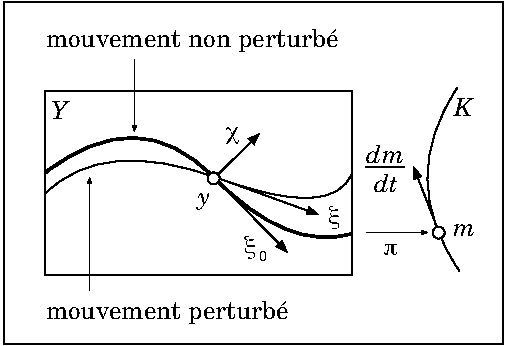
\includegraphics{Figures/IglesiasFig3.pdf}}
    \caption{Projection de $Y$ sur $\mathcal{K}$}\label{figure3}
  \end{figure}
  %###########
  
  Considérons alors une feuille du feuilletage $y\mapsto \RR\cdot \xi$ passant par $y=(t,\rr,\vv)$.
  Cette courbe se projette sur l'espace des mouvements képleriens $\mathcal{K}$,
  son équation est alors :
  %
  \begin{equation}
    \frac{dm}{dt} = D\pi_y(\xi)=D\pi_y(\xi_0) + D\pi_y(\chi),
  \end{equation}
  %
  où $\pi : y\mapsto m$ est la projection de $Y$ sur son quotient et $D$ désigne l'application linéaire tangente.
  Or,
  par construction :
  $D\pi_y(\xi_0)=0$,
  il reste donc $dm/dt= D\pi_y(\chi)$.
  Un petit dessin vaut parfois mieux qu'un long discours,
  voir figure \ref{figure3}.
  C'est la famille d'équations (\ref{eq_B}).
  Enfin,
  transformée en la famille d'équations (\ref{eq_C}),
  elle s'écrit encore :
  %
  \begin{equation}
    \frac{dm}{dt} = \omega^{-1}(d\Omega),
  \end{equation}
  %
  où $d\Omega$ désigne la différentielle de $\Omega$.
  Par analogie avec le cas euclidien,
  comme $\omega$ est inversible,
  on appelle \emph{gradient symplectique} de la fonction $\Omega$ le champ de vecteurs $\omega^{-1}(d\Omega)$.
  L'équation différentielle qui décrit la variation des constantes devient après ces conventions de langage :
  %
  \begin{equation}
    \frac{dm}{dt} = \operatorname{grad}(\Omega).
  \end{equation}
  %
  L'évolution du mouvement $m$,
  perturbé par le potentiel $\Omega$,
  est donc la courbe intégrale du gradient symplectique du potentiel de perturbation.
  
  %*****
  \section*{Conclusion}
  
  La partie la plus douteuse du travail de Lagrange concerne sûrement la méthode d'approximation utilisée.
  Je voudrais à ce propos souligner qu'hormis ces méthodes d'approximation les conclusions de Lagrange sont rigoureusement établies même si la présentation qu'il en a faite,
  et que j'ai essayé de reproduire ici,
  ne respecte pas les canons actuels de la mathématique.
  En ce sens,
  les transformations qu'il apporte aux équations initiales ne sont pas d'une grande utilité puisque celles qu'il obtient leur sont absolument équivalentes.
  Laissons-le parler :
  %
  \begin{quote}
    \og Ainsi on peut regarder les équations précédentes entre les nouvelles variables $a$, $b$, $c$, etc. comme les transformées des équations en $x$, $y$, $z$ ; mais ces transformations seraient peu utiles pour la solution générale du problème. Leur grande utilité est lorsque la solution rigoureuse est impossible, et que les forces perturbatrices sont très petites ; elles fournissent alors un moyen d'approximation.\fg{}.
  \end{quote}
  %
  Mais la justification de ces méthodes emploiera un grand nombre de mathématiciens après lui et non des moindres.
  Poincaré soulignait dans l'introduction de sa célèbre \emph{Nouvelle mécanique céleste} \cite{Poincare1} :
  %
  \begin{quote}
    \og Ces méthodes qui consistent à développer les coordonnées des astres suivant les puissances des masses, ont en effet un caractère commun qui s'oppose à leur emploi pour le calcul des éphémérides à longue échéance. Les séries obtenues contiennent des termes dits \emph{séculaires}, où le temps sort des signes des sinus et cosinus, et il en résulte que leur convergence pourrait devenir douteuse si l'on donnait à ce temps $t$ une grande valeur.
    
    La présence de ces termes séculaires ne tient pas à la nature du problème, mais seulement à la méthode employée. Il est facile de se rendre compte, en effet, que si la véritable expression d'une coordonnée contient un terme en $\sin \alpha mt$, $\alpha$ étant une constante et $m$ l'une des masses, on trouvera quand on voudra développer suivant les puissances de $m$, des termes séculaires $\alpha mt - \alpha^3m^3t^3/6 +\cdots$ et la présence de ces termes donnerait une idée très fausse de la véritable forme de la fonction étudiée.\fg{}
  \end{quote}
  %
  Cette objection est sans nul doute très pertinente et a conduit,
  notamment grâce aux travaux de Poincaré,
  au développement de la géométrie symplectique -- en particulier en ce qui concerne son application à la mécanique.
  De nouvelles théories sont nées comme par exemple la théorie des systèmes complètement intégrables et de leur perturbation qui a donné le fameux théorème\footnote{Théorème difficile.} de Kolmogorov -- Arnold -- Moser,
  sur la stabilité de nombreux mouvements après perturbation (voir \cite{Arnold0} \cite{Arnold1})
  
  \bigskip
  
  %###########
  \begin{figure}[p]
    \centerline{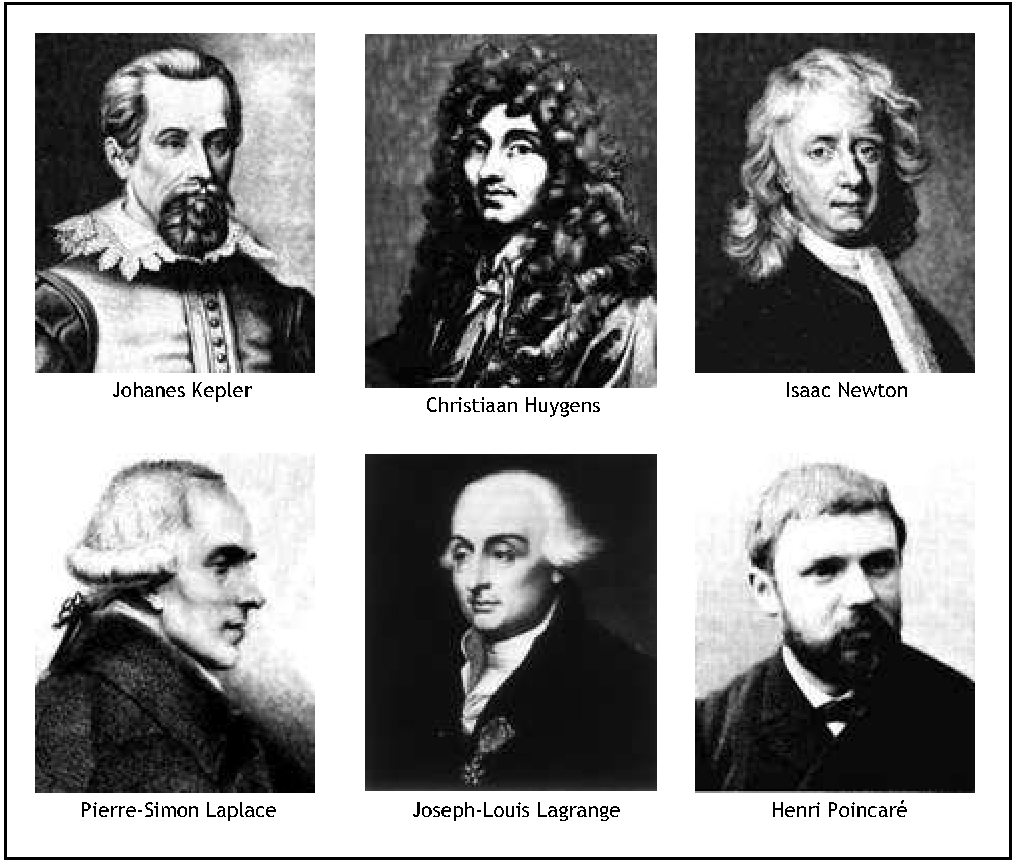
\includegraphics{Figures/portraits.pdf}}
    \caption{Galerie des portraits}\label{portraits}
  \end{figure}
  %###########
  
  \begin{thebibliography}{Sou86}
    
    \bibitem[Arn76]{Arnold0}
    V.~I. Arnold.
    \newblock {\em Méthodes mathématiques de la mécanique classique}.
    \newblock Éditions MIR, Moscou, 1976.
    
    \bibitem[Arn80]{Arnold1}
    V.~I. Arnold.
    \newblock {\em Chapitres supplémentaires à la théorie des équations différentielles}.
    \newblock MIR, Moscou, 1980.
    
    \bibitem[dG87]{deGandt1}
    F.~de~Gandt.
    \newblock Force et géométrie.
    \newblock Thèse de doctorat, Paris I, 1987.
    
    \bibitem[Lag74]{Lagrange5}
    J.-L. Lagrange.
    \newblock Sur les intégrales particulières des équations différentielles.
    \newblock Dans {\em \OE uvres de Lagrange}, volume~IV, page 5.
    Gauthier-Villars, Paris, 1877.
    \newblock Nouveaux Mémoires de l'Académie royale des Sciences et Belles Lettres de Berlin, année 1774.
    
    \bibitem[Lag75]{Lagrange6}
    J.-L. Lagrange.
    \newblock Recherches sur Les suites récurrentes.
    \newblock Dans {\em \OE uvres de Lagrange}, volume~IV, page 151.
    Gauthier-Villars, Paris, 1877.
    \newblock Nouveaux Mémoires de l'Académie royale des Sciences et Belles Lettres de Berlin, année 1775.
    
    \bibitem[Lag79]{Lagrange7}
    J.-L. Lagrange.
    \newblock Sur différentes questions d'analyse relatives à la théorie des intégrales particulières.
    \newblock Dans {\em \OE uvres de Lagrange}, volume~IV, pages 585.
    Gauthier-Villars, Paris, 1877.
    \newblock Nouveaux Mémoires de l'Académie royale des Sciences et Belles Lettres de Berlin, année 1779.
    
    \bibitem[Lag08]{Lagrange2}
    J.-L. Lagrange.
    \newblock Sur la théorie des variations des éléments des planètes et en particulier des variations des grands axes de leurs orbites.
    \newblock Dans {\em \OE uvres de Lagrange}, volume~VI, pages 713--768.
    Gauthier-Villars, Paris, 1877.
    \newblock Lu, le 22 août 1808 à l'Institut de France.
    
    \bibitem[Lag09]{Lagrange3}
    J.-L. Lagrange.
    \newblock Sur la théorie générale de la variation des constantes arbitraires dans tous les problèmes de la mécanique.
    \newblock Dans {\em \OE uvres de Lagrange}, volume~VI, pages 771--805.
    Gauthier-Villars, Paris, 1877.
    \newblock Lu, le 13 mars 1809 à l'Institut de France.
    
    \bibitem[Lag10]{Lagrange4}
    J.-L. Lagrange.
    \newblock Second mémoire sur la théorie générale de la variation des constantes arbitraires dans tous les problèmes de la mécanique.
    \newblock Dans {\em \OE uvres de Lagrange}, volume~VI, pages 809--816.
    Gauthier-Villars, Paris, 1877.
    \newblock Lu, le 19 février 1810 à l'Institut de France.
    
    \bibitem[Lag11]{Lagrange1}
    J.-L. Lagrange.
    \newblock {\em Mécanique analytique}.
    \newblock Librairie Albert Blanchard, Paris, 1965.
    \newblock Fac-similé de la troisième édition.
    
    \bibitem[Poi92]{Poincare1}
    Henri Poincaré.
    \newblock {\em Les nouvelles méthodes de la mécanique céleste}.
    \newblock Gauthier-Villars, Paris, 1892.
    
    \bibitem[Sou53]{Souriau20}
    J.-M. Souriau.
    \newblock Géométrie symplectique différentielle. Applications.
    \newblock {\em Coll. Int. CNRS}, p. 53, Strasbourg 1953.
    
    \bibitem[Sou86]{Souriau9}
    J.-M. Souriau.
    \newblock La structure symplectique de la mécanique décrite par lagrange en 1811.
    \newblock {\em Math. Sci. hum.}, (94): 45--54, 1986.
    
    \bibitem[Ste69]{Sternberg1}
    S.~Sternberg.
    \newblock {\em Celestial Mechanics}.
    \newblock W. A. Benjamin Inc., New--York, 1969.
    
    \bibitem[Wey46]{Weyl1}
    H.~Weyl.
    \newblock {\em The Clasical Groups, their Invariants and Representations}.
    \newblock Princeton University Press, New-Jersey, Princeton 1946.
    
  \end{thebibliography}
  
\end{document}
